\documentclass{article}
\usepackage{graphicx}
\usepackage{multirow}

\title{Predicting Car MSRP Using Ensemble Methods}
\author{Karlo Papa & Josh Wong}
\date{December 14, 2023}

\begin{document}

\maketitle

\begin{abstract}
This study presents a multi-faceted approach to predicting car Manufacturer's Suggested Retail Price (MSRP) using a variety of popular indicators. We use both categorical and continuous indicators in our regression and classification tasks. Our research in understanding the determinants of MSRP is pertinent to the rapidly evolving automotive sector. The U.S. alone boasts an impressive fleet of approximately 286 million vehicles, encompassing a diverse range of 383 automotive brands. We leverage a dataset sourced from Kaggle comprising various car attributes along with the cars MSRP. The objective of this study is to present a comprehensive approach to understanding and predicting MSRPs of cars based on specific features by weighing their importance to generate an equitable value. By diving into the intricate branch of values, we aim to empower customers, manufacturers, and dealers with a profit-making understanding of what forces shape the price tags of automobiles. 

\end{abstract}



\section{Introduction}




Past research has been conducted predicting the resale price of used cars. This research mainly relies on two indicators: mileage and age. We attempt to predict the MSRP of cars which is their value when they are new. We use a more diverse set of indicators to get the full picture of what makes a car valuable — providing value to car manufacturers and consumers. The United States boasts a staggering fleet of approximately 286 million vehicles, spread across 383 automotive brands. This unprecedented diversity presents a unique challenge in predicting vehicle pricing. To tackle this challenge we employ a dataset sourced from Kaggle which contains a wide spectrum of continuous and binary car attributes over many instances. We employ the use of ensemble methods in both regression and classification tasks to accurately predict the MSRP of cars with given indicators. 
\newline
\newline
Our ensembles are built off of Naive Bayes, Random Forest, Linear Regression, Random Forest Regressor, and Decision Tree Regressor algorithms. Our ensemble models were able to accurately predict car MSRP using evaluation metrics such as accuracy, mean squared error (MSE), and F1 score. We employed various methods to improve our models by tuning the models, adjusting the features, and adjusting our buckets. This resulted in our regression ensemble and our modified bucket classification model exhibiting remarkable results. In summary, this project contributes not only to the existing body of knowledge in automotive pricing strategies but develops new frameworks for valuing new cars and their features.

\begin{figure}[h]
\caption{Improved Classification Ensemble Results}
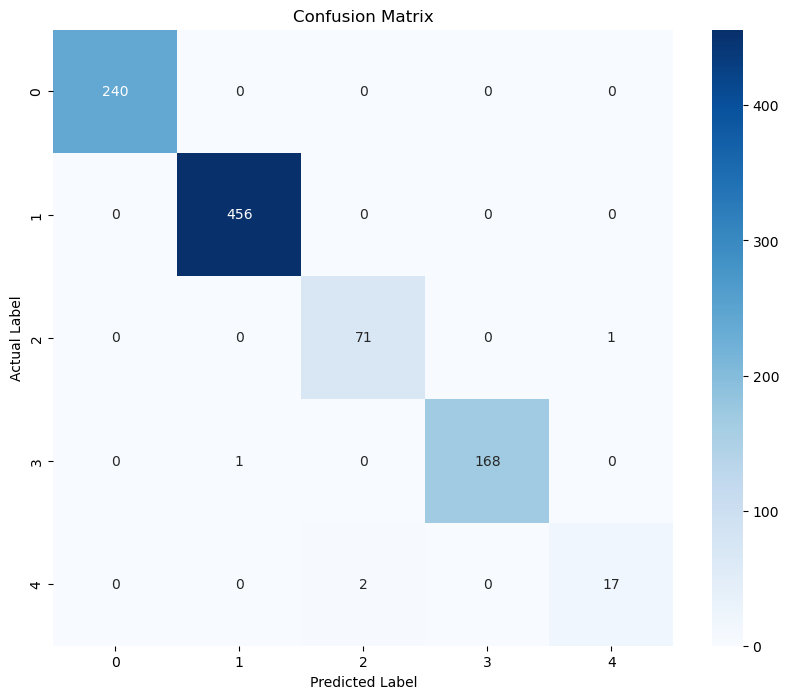
\includegraphics[scale=0.5]{Simplified Matrix by string class.png}\newline
\end{figure}

\begin{table}[h]
\centering
\caption{Ensemble Regression Results}
\vspace{3pt}
\label{tab:hyperparameters}
\begin{tabular}{|l|l|l|}
\hline
\textbf{Hyperparameter} & \textbf{R Squared} & \textbf{Mean Squared Error} \\
\hline
Ensemble Regression & 0.907 & 102711195 \\
\hline
Ensemble Regression exclude 100k+ & 0.867 & 37437977 \\
\hline
\end{tabular}
\end{table}

\section{Problem Description}
In this study, we addressed the intricate task of predicting the Manufacturer's Suggested Retail Price (MSRP) of new cars. Unlike previous research that focused primarily on predicting the resale value of used cars using limited indicators like mileage and age, our approach expands the scope to include a more diverse set of indicators. The learning problem here involves both regression and classification tasks. The regression aspect aims to predict the MSRP as a continuous variable, while the classification task categorizes cars into different price ranges based on their features.
\newline
\newline
Our analysis utilized a comprehensive dataset sourced from Kaggle, which includes a wide array of car attributes, both continuous and binary, along with the cars' MSRP. The dataset encompasses data as summarized in the following tables. This diversity in data offers a unique opportunity to explore and understand what attributes contribute to the new value of a car.
\newline
\newline
We aim to provide valuable insights to car manufacturers and consumers by identifying the key features that determine the MSRP of new cars. Understanding these factors can aid manufacturers in pricing strategies and feature prioritization, while consumers can benefit by making more informed purchasing decisions. Additionally, this research contributes to the academic field by developing frameworks for valuing new cars and their features, extending beyond the traditional focus on used car pricing. With more transparency in the car market, manufacturers can better create the cars consumers want at the prices consumers are willing to pay.
\newline
\newline
To address this complex problem, we employed a regression and classification ensemble method. Our classification ensemble method used the Naive Bayes and Random Forest methods, while our regression ensemble used the Linear Regression, Random Forest Regressor, and Decision Tree Regressor algorithms. Our approach involved using these models to accurately predict the MSRP based on a comprehensive set of car attributes. We then evaluated our models' performance based on a variety of performance attributes using metrics such as accuracy, mean squared error (MSE), and F1 score. We continuously refined our models by tuning hyperparameters, adjusting features, and modifying classification buckets. This iterative process of improvement and validation led to our regression ensemble and modified bucket classification model exhibiting remarkable predictive capabilities.



\section{Approaches}

In this section we outline the approaches we employed to accurately predict the MSRP of cars based on a variety of indicators. The process commenced with feature selection and the development of a short decision tree, followed by the application of both classification and regression models. First, the initial columns such as ‘make’, ‘model’, and ‘year’ were removed to ensure brand independence and enhance the utility of results for both consumers and producers. 

\subsection{Decision Tree}
We constructed a decision tree with a maximum depth of 4 and one with max depth 5. These models aimed to identify the attributes most indicative of MSRP and then build a framework to classify MSRP into buckets. Key indicators identified include engine horsepower (HP), market category, engine fuel type, popularity, and the number of doors. Higher engine HP, luxury market category, diesel fuel type, less popularity, and fewer doors were associated with higher MSRPs. We noticed that certain parameters, such as two doors, were divided between luxury and budget. For example, a two door car could either be an expensive Ferrari or a standard Ford. In short, the decision tree was used to identify key indicators for MSRP and provided foundational insights for subsequent analyses. \newline

\subsection{Regression Ensemble Architecture and Rationale}

\subsubsection{Model Building}
\begin{itemize}
\item \textbf{RandomForestRegressor} Chosen for its robustness and ensemble approach that combines multiple decision trees to reduce variance and prevent overfitting.
\\
\item \textbf{DecisionTreeRegressor} Provides interpretability and captures non-linear patterns, beneficial in understanding feature influence on MSRP.
\\
\item \textbf{LinearRegression} Offers a baseline model for linear relationships, important for capturing straightforward, additive feature effects on MSRP.

\end{itemize}
\subsubsection{Ensemble Creation}
Voting Regressor implements hard/soft voting to classify instances. In the 'hard voting' approach, the final classification is determined by the majority vote from all models. Conversely, 'soft voting' considers the probability estimates from each model, averaging them to decide the final classification.

\subsubsection{Rationale}
The chosen architecture blends complexity with simplicity. The `RandomForestRegressor` is a powerful model that can handle a variety of data types and distributions, making it a versatile choice for the ensemble. It's particularly effective in a dataset with many features, as it can capture interactions between them without the need for explicit feature engineering. 
\newline 
\newline
The `DecisionTreeRegressor` is included for its ability to make clear, hierarchical decisions based on the data, providing insights into the importance of various features in predicting MSRP. This can be particularly useful for interpretability—a key aspect when stakeholders might require an explanation of the model's predictions. Lastly, `LinearRegression` is used for its speed and interpretability in establishing a baseline for performance. It’s excellent for capturing linear relationships and serves as a counterbalance to the more complex models in the ensemble, ensuring that simple, yet significant, relationships are not overlooked.

\subsubsection{Overview}
Our ensemble method synergizes three distinct regression models into a cohesive predictive framework. The ensemble employs a `VotingRegressor`, which averages the individual predictions to produce a final estimate. In the 'hard voting' approach, the final classification is determined by the majority vote from all models. Conversely, 'soft voting' considers the probability estimates from each model, averaging them to decide the final classification. This dual approach leverages the strengths of each model, enhancing the ensemble's predictive accuracy and robustness. 
\newline
\newline 
RandomForestRegressor uses its ensemble learning approach to mitigate overfitting. Our LinearRegression model forecasts continuous outcomes by capturing linear relationships between variables. Finally, a DecisionTreeRegressor maps out complex, non-linear interactions within the dataset. By combining these models our ensemble offers a balanced and comprehensive prediction of car MSRPs, enhancing the precision of our estimates while accounting for a spectrum of influences on a vehicle's market value.

\subsection{Classification Ensemble Architecture and Rationale}
\subsubsection{Model Building}
\begin{itemize}
    \item \textbf{RandomForestClassifier} Selected for its high accuracy and capability to manage overfitting through its ensemble of decision trees.
    \item \textbf{GaussianNB (Naive Bayes)} Introduced in the second iteration for its simplicity and effectiveness in handling large datasets with a probabilistic approach.
    \item \textbf{DecisionTreeClassifier} Utilized initially for its simplicity and interpretability, capturing complex decision rules effectively.
\end{itemize}
\subsubsection{Ensemble Creation}
\begin{itemize}
    \item \textbf{VotingClassifier} Implements hard/soft voting to classify instances. In the 'hard voting' approach, the final classification is determined by the majority vote from all models. Conversely, 'soft voting' considers the probability estimates from each model, averaging them to decide the final classification.
\end{itemize}
\subsubsection{Rationale}
We designed our ensemble to leverage the complementary strengths of the classifiers. The RandomForestClassifier is adept at handling non-linear relationships and interactions. The initial use of the DecisionTreeClassifier provided clear, interpretable decision-making insights. In our second iteration, we introduced GaussianNB for its efficient handling of probability distributions, making it valuable in predicting categorical outcomes like MSRP bins. We utilized LogisticRegression paired with StandardScaler in a pipeline to standardize feature scales and mitigate bias in model predictions.
\newline
\subsubsection{Overview}
We employed an ensemble method for classification, integrating a trio of models to predict car MSRPs binned into categories. A VotingClassifier aggregated the verdicts from individual models to yield a final classification based on two approaches. In the 'hard voting' approach, the final classification is determined by the majority vote from all models. Conversely, the 'soft voting' approach considered the probability estimates from each model, averaging them to decide the final classification. This dual approach leveraged the strengths of each model, enhancing the ensemble's predictive accuracy and robustness.
\newline
\newline
Our ensemble's foundation is a RandomForestClassifier which is particularly resistant to overfitting, despite the complexity of our dataset. Additionally, we used a DecisionTreeClassifier to bring simplicity to our model and results. To complete the first model we implemented a LogisticRegression model which operates within a pipeline that standardizes features, ensuring consistent contribution across all variables. Our ensemble works together with RandomForestClassifier handling the dataset's intricacies, the DecisionTreeClassifier simplifying the decision process, and the LogisticRegression offering a solid baseline for comparison.
\newline
\newline
In our second iteration we replaced the DecisionTreeClassifier with the GaussianNB (Naive Bayes) model. This model complements the ensemble by providing a different perspective on classification, leveraging its strength in probabilistic reasoning. It's particularly useful in our scenario for predicting categorical outcomes, like MSRP bins, based on a broad set of features. The inclusion of GaussianNB aimed to capture subtleties in the data that other models might overlook.
\newline
\section{Experimental Setup}

\subsection{Data Sources}
Our study utilized a comprehensive dataset titled "Car Features and MSRP," sourced from Kaggle and compiled from Edmunds and Twitter. This dataset includes various car attributes such as make, model, year, engine type, and other features crucial for MSRP prediction. The features are summarized in the table below:

\begin{table}[ht]
\centering
\caption{Raw Features Data Set}
\vspace{3pt}
\begin{tabular}{|l|c|}
\hline
\textbf{Description} & \textbf{Value} \\
\hline
Number of Indicators & 16 \\
Number of Categorical Features & 8 \\
Number of Continuous Features & 8 \\
Number of Instances & 11,914 \\
Years Observed & 27 \\
\hline
\end{tabular}
\label{tab:raw_features_info}
\end{table}

\begin{table}[ht]
\centering
\caption{Features Data Set Post Processing}
\vspace{3pt}
\begin{tabular}{|l|c|}
\hline
\textbf{Description} & \textbf{Value} \\
\hline
Number of Indicators & 14 \\
Number of Categorical Features & 6 \\
Number of Continuous Features & 8 \\
Number of Instances & 4,776 \\
Years Observed & 4 \\
\hline
\end{tabular}
\label{tab:features_info}
\end{table}
\subsection{Preprocessing}
We focused on removing missing values and ensuring our data wasn’t influenced by inflation. Additionally we optimized categorical variables to combine classes that meant the same thing and to reduce the total number of classes within each indicator. Our process is outlined below:

\begin{enumerate}

    \item Dataset Diagnostics
    \begin{itemize}
        \item Objective: Understand underlying data characteristics.
        \item Method: Perform exploratory data analysis (EDA) to assess distribution, identify outliers, and understand the dataset’s structure. This step is essential for informed preprocessing and modeling decisions.
    \end{itemize}

    \item Handling Missing Values:
    \begin{itemize}
        \item Objective: Ensure data completeness and reliability.
        \item Method: Rows with any missing or 'N/A' values are dropped. This step is crucial to ensure our data is full for training and to prevent inaccuracies in the analysis and model training.
    \end{itemize}
    
    \item Year Filter:
    \begin{itemize}
        \item Objective: Focus the analysis on recent car models.
        \item Method: Filter the dataset to include only cars from the years 2014-2017. This temporal focus ensures that the analysis is relevant to current market trends and consumer preferences. Also keeping the year selection short means inflation won't be able to skew our results.
    \end{itemize}

    \item Door Count Filter:
    \begin{itemize}
        \item Objective: Optimize door count indicator.
        \item Method: Exclude cars that do not have 2 or 4 doors, thereby focusing on the most common and commercially significant segments of the automotive market.
    \end{itemize}
    
    \item Drive Type Adjustment:
    \begin{itemize}
        \item Objective: Simplify transmission categories.
        \item Method: Remove 'Direct Drive' transmission types as they might represent a niche market. Combine 'Automated Manual' with 'Manual' to reduce category fragmentation.
    \end{itemize}
    
    \item Drive System Consolidation:
    \begin{itemize}
        \item Objective: Streamline drive system categories.
        \item Method: Merge 'Four Wheel Drive' (4WD) and 'All Wheel Drive' (AWD) into a single category to simplify analysis and address potential overlaps.
    \end{itemize}
    
    \item Fuel Type and Basic Information:
    \begin{itemize}
        \item Objective: Focus on meaningful attributes for regression.
        \item Method: Group similar fuel types to reduce complexity. Remove nominal variables like 'Make', 'Model', and 'Year', as they might not contribute significantly to a numerical regression analysis and we do not want our factors influenced by branding.
    \end{itemize}
    
    \item Market Categories and Vehicle Styles:
    \begin{itemize}
        \item Objective: Generalize vehicle classifications.
        \item Method: Simplify these categories into broader groups to facilitate a more generalized analysis, reducing the impact of niche market variations. Additionally, ensure every car has only one market category.
    \end{itemize}
    
    \item Engine Cylinders Filter:
    \begin{itemize}
        \item Objective: Concentrate on common engine configurations.
        \item Method: Limit the dataset to cars with 4, 6, or 8 cylinders, focusing on the most prevalent and market-relevant engine types.
    \end{itemize}
    
    \item Binning Continuous Variables:
    \begin{itemize}
        \item Objective: Manage non-linear relationships in continuous data.
        \item Method: Convert continuous variables into categorical bins. This allows us to employ classification techniques across all indicators.
    \end{itemize}
    
    \item Categorical Variables for Regression:
    \begin{itemize}
        \item Objective: Enhance regression analysis efficiency.
        \item Method: Exclude categorical variables from the regression model to focus solely on numerical predictors.
    \end{itemize}
    
    \item Price Cap:
    \begin{itemize}
        \item Objective: Target a broader consumer base.
        \item Method: Exclude ultra-luxury cars by removing those priced over \$100,000, ensuring the model is applicable to a wider range of typical consumers. This price cap helps align the analysis with the purchasing power and preferences of the majority of car buyers.
    \end{itemize}

    \item Manual Categorization:
    \begin{itemize}
        \item Objective: Incorporate “best judgment” into categorization.
        \item Method: Manually classify cars into 5 distinct buckets based on distribution and general knowledge of the car market. This adds a layer of qualitative analysis that complements the quantitative approach.
    \end{itemize}
    
\end{enumerate}

\subsection{Decision Tree}
We developed a decision tree that served as a foundational tool for understanding the key attributes that influence a car's MSRP. We created decision trees with maximum depths of 4 and 5, aiming to identify the most significant indicators for new car pricing. This process highlighted several critical indicators, such as engine horsepower (HP), market category, engine fuel type, popularity, and the number of doors. We encoded categorical variables using OneHotEncoder, transforming them into a format suitable for the decision tree algorithm. We set sparse=False and handle\_unknown='ignore' in the encoder to effectively manage unknown categories and improve matrix efficiency. The resulting encoded categorical data was then combined with the numerical data to form a comprehensive feature set.
\newline
\newline
We utilized the DecisionTreeRegressor from scikit-learn, with a maximum depth of 4 and a random state of 42 to maintain consistent results across various runs. This model was then trained on the training data. This rigorous approach in data preprocessing and model training allowed us to reliably identify the key attributes influencing a car's MSRP, ensuring the robustness of our analysis.For training and validation, we split this combined data into a training set and a testing set, allocating 20\% of the dataset for testing. We ensured reproducibility in our experiment by setting a random state of 42 during the splitting process. \newline
The decision tree's insights provided a starting point for our further analysis, allowing us to understand the complexities of car pricing and laying the groundwork for more advanced predictive models.

\subsection{Ensemble Regression}
We developed an ensemble regression method to accurately predict car Manufacturer's Suggested Retail Prices (MSRPs). This approach combined multiple predictive algorithms to enhance effectiveness. The process began with splitting the dataset into training and testing sets, designating 20\% for testing. We then applied the StandardScaler to the features, ensuring uniformity in scale across all variables and eliminating any bias towards higher magnitude variables.
\newline
\newline
Our ensemble model was configured to integrate three distinct algorithms. The RandomForestRegressor was set with 200 estimators and a maximum depth of 20. It captured complex, non-linear relationships and mitigated overfitting. The DecisionTreeRegressor, with a maximum depth of 10, provided in-depth insights into how various features influenced the MSRP, capturing intricate data patterns. LinearRegression served as a baseline model, elucidating linear relationships between features and the target variable.
\newline
\newline
We then combined these models into a VotingRegressor ensemble, leveraging the unique strengths of each to achieve solid predictive accuracy. The ensemble model was trained on the scaled training data, ensuring a robust learning process. The ensemble model was then evaluated on the test set, utilizing performance metrics such as Mean Squared Error (MSE) and R-squared to gauge accuracy and fit. Our ensemble regression approach was effective at understanding the relationships within our data, resulting in accurate and reliable MSRP predictions. 
\newline
\newline
Additionally we ran a regression on data excluding cars with MSRP over 100,000 to target the general population. We thought that by excluding supercars we could maybe create a better model for the average consumer.

\subsection{Ensemble Classification}
Our classification ensemble included a RandomForestClassifier, optimized with 200 estimators and a max depth of 20, a DecisionTreeClassifier with a max depth of 10, and a Logistic Regression model with a regularization strength of 1 and 500 maximum iterations. These models were selected for their individual strengths in handling complex data structures and relationships.
\newline
\newline
We preprocessed the dataset using LabelEncoder for categorical features and split it into training and testing sets, allocating 20\% for testing. The StandardScaler was employed for feature scaling, particularly for the Logistic Regression model. Our classifier ensembles were constructed using a VotingClassifier, some had a 'hard voting' mechanism and others had a 'soft voting' mechanism. In the 'hard voting' approach, the final classification is determined by the majority vote from all models. Conversely, 'soft voting' considers the probability estimates from each model, averaging them to decide the final classification. This ensemble combined the strengths of RandomForestClassifier, DecisionTreeClassifier, and Logistic Regression, integrated through a pipeline with feature scaling.
The model was trained on the scaled training data and evaluated on the test set. Performance was assessed using a confusion matrix, providing insights into the model's predictive accuracy and classification efficacy. This ensemble classification approach proved effective in accurately categorizing cars into different MSRP ranges, leveraging the diverse capabilities of the included models.
\newline
\newline
We modified our final ensemble classification by manually binning MSRP. We placed the MSRP into five bins based on “Budget,” “Economy,” “Luxury,” “Performance,” and “Supercar.” We manually created these bins using prior knowledge of car classes and the distribution of our MSRP data. We hope this classification will be more useful to consumers and manufacturers because they just need general classification. In addition we hope this manual split will improve model performance.

\subsection{Performance Measures}
To evaluate the performance of our models, we used several key metrics.

For our regression models, we used:
\begin{itemize}
    \item Mean Squared Error: This metric helped us gauge the accuracy of our predictions, providing insight into the average distance of the predicted values from the actual values.
    \item R Squared (R²): R² measured the proportion of variance in the dependent variable that could be predicted from the independent variables. This was crucial in assessing the model's explanatory power.
\end{itemize}

For our classification models, we utilized a comprehensive set of metrics:
\begin{itemize}
    \item Accuracy: This indicated the proportion of correctly predicted instances, offering a straightforward measure of overall model performance.
    \item F1 Score: By balancing precision and recall, the F1 Score provided a more nuanced view of model performance, especially in datasets with an uneven class distribution.
    \item Area Under the Curve (AUC): The AUC of the Receiver Operating Characteristic (ROC) curve, helped evaluate the true positive rate against the false positive rate, providing an aggregate measure of performance across various threshold settings.
    \item Confusion Matrices: These matrices presented a detailed breakdown of correct and incorrect classifications, allowing us to understand the model's performance across different classes.
\end{itemize}

Together, these metrics offered a comprehensive evaluation of our models, with Squared Error and R² shedding light on the regression models' predictive accuracy, while Accuracy, F1 Score, AUC, and Confusion Matrices provided in-depth insights into the classification models' effectiveness.
\newline
\newline
Additionally, we used confusion matrices to evaluate the performance of our classification models. This was especially useful when considering our application of these models. Consumers don't necessarily care about small differences in price - they are just looking for a certain “range” of car. So when we were classifying into the 10 MSRP buckets, our performance measures didn’t appear great, but the confusion matrices revealed that our models were classifying within one class of the correct class, so our models were performing generally well.





\section{Experimental Results}
Our models produced significant results that were effective in reaching the objectives they set out to achieve. Our ensemble regression and decision tree were effective without much optimization. We were able to optimize our classification through a variety of ways. We substituted DecisionTreeClassifier for GaussianNB, and then manually separated our MSRP into buckets. This resulted in a very accurate classification.

\subsection{Decision Tree}
Our decision trees are included in the appendix, the main takeaways are that Engine Horsepower (HP) is a significant predictor, with higher HP pointing to a higher price tag. The market category notably impacts the car's cost, particularly distinguishing between luxury and non-luxury models, with luxury ones commanding a higher price. The type of fuel a car uses is relevant too; diesel cars tend to be more expensive. A vehicle's popularity inversely relates to its price—less popular models are usually pricier. Lastly, the number of doors is a price indicator; cars with fewer doors are often on the higher end of the price spectrum.

\subsection{Ensemble Regression}
Table 4 outlines our Ensemble Regression results. The regression trained on the whole dataset performed better than the regression trained on the dataset excluding cars over 100k MSRP.

\begin{table}[h]
\centering
\caption{Ensemble Regression Results}
\vspace{3pt}
\label{tab:hyperparameters}
\begin{tabular}{|l|l|l|}
\hline
\textbf{Hyperparameter} & \textbf{R Squared} & \textbf{Mean Squared Error} \\
\hline
Ensemble Regression & 0.907 & 102711195 \\
\hline
Ensemble Regression exclude 100k+ & 0.867 & 37437977 \\
\hline
\end{tabular}
\end{table}

\subsection{Ensemble Classification}
The results of our Ensemble Classification are shown in the following figures and tables.
\newline
\newline
Table 5 shows the Ensemble Classification results trained on the 10 buckets condensed in a table. Table 6 shows the Ensemble Classification results trained on the manual buckets condensed in a table.
\newline
\newline
Figures 2-6 show the confusion matrices for our Ensemble Classification. Figure 6 shows the confusion matrix for our model when tested on the manual buckets. Figure 8 shows the ROC for the 10 bucket model, with figure 9 showing the ROC for the manual bucket model. The manual bucket model performed much better.



\begin{table}[h]
\centering
\caption{Ensemble Classification 10 Bin Results}
\vspace{3pt}
\label{tab:hyperparameters}
\begin{tabular}{|l|l|l|l|l|}
\hline
\textbf{Hyperparameter} & \textbf{Precision} & \textbf{Recall} & \textbf{f1-score} & \textbf{Support} \\


\hline
0 & 0.76 & 0.72 & 0.74 & 92 \\
\hline
1  & 0.40 & 0.43 & 0.42 & 90 \\
\hline
2 & 0.39 & 0.36 & 0.37 & 95 \\
\hline
3  & 0.34 & 0.32 & 0.33 & 93 \\
\hline
4 & 0.34 & 0.38 & 0.36 & 92 \\
\hline
5 & 0.41 & 0.42 & 0.42 & 103 \\
\hline
6 & 0.44 & 0.44 & 0.44 & 93 \\
\hline
7 & 0.64 & 0.57 & 0.60 & 105 \\
\hline
8  & 0.70 & 0.76 & 0.73 & 99 \\
\hline
9 & 0.87 & 0.89 & 0.88 & 94 \\
\hline
macro avg & 0.53 & 0.53 & 0.53 & 956 \\
\hline
\end{tabular}
\end{table}

\begin{table}[h]
\centering
\caption{Ensemble Classification 10 Bin Results}
\vspace{3pt}
\label{tab:hyperparameters}
\begin{tabular}{|l|l|l|l|l|}
\hline
\textbf{Hyperparameter} & \textbf{Precision} & \textbf{Recall} & \textbf{f1-score} & \textbf{Support} \\
\hline
      budget &     1.00 &     1.00 &     1.00  &     240 \\
      \hline
     economy &      1.00 &     1.00 &     1.00  &     456 \\
     \hline
      luxury &      0.97 &     0.99 &     0.98  &      72 \\
      \hline
    performance &      1.00 &     0.99 &     1.00   &    169 \\
     \hline
    supercar &      0.94 &     0.89 &     0.92  &      19 \\
    \hline
   macro avg &      0.98 &     0.97 &     0.98 &      956 \\
   

\hline
\end{tabular}
\end{table}




\begin{figure}[htbp]
    \centering
    
    
    \begin{minipage}{\textwidth}
        \centering
        \caption{Hard Voting Confusion Matrix}
        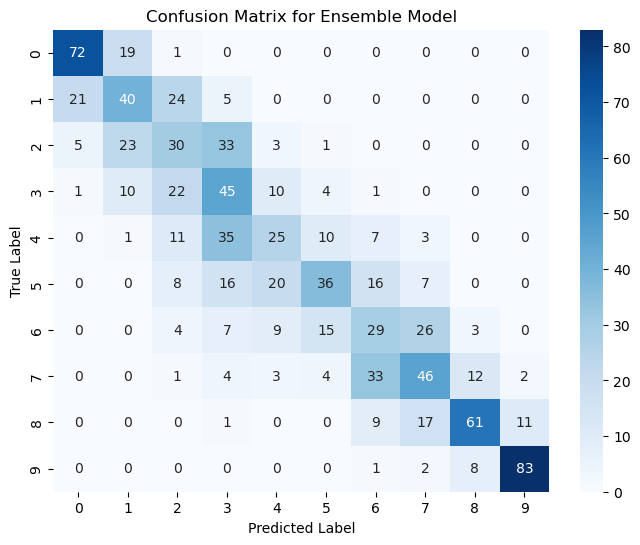
\includegraphics[scale=0.5]{ConfusionMAtrixHardClassVoting.png}
    \end{minipage}
    Confusion Matrix for Ensemble Model (Hard Voting): The confusion matrix visualizes the performance of an ensemble model employing hard voting. It contrasts the actual labels with the predicted ones, documenting correct and incorrect classifications numerically.

    
    \begin{minipage}{\textwidth}
        \centering
        \caption{Soft Voting Confusion Matrix}
        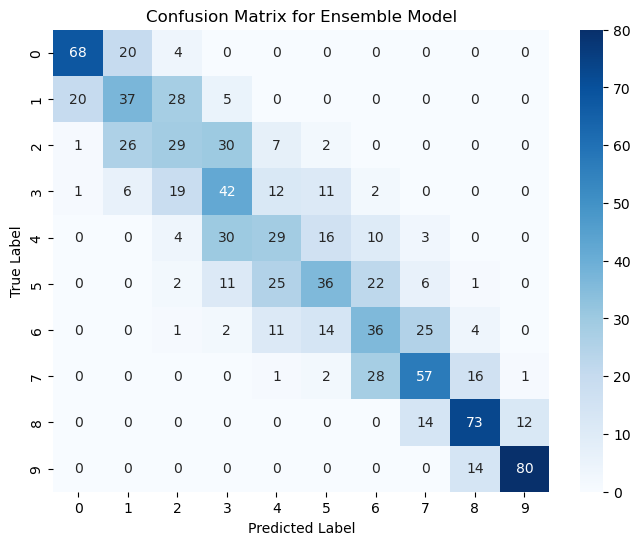
\includegraphics[scale=0.5]{ConfusionMAtrixSoftClassVoting.png}
    \end{minipage}
    Confusion Matrix for Ensemble Model (Soft Voting): This confusion matrix, associated with soft voting in an ensemble model, compares predicted labels against true labels to assess the model's predictive performance, potentially across different prediction sets or validation folds.
 \caption{Multiple Figures}
\end{figure}

\begin{figure}[htbp]
    \centering

      \begin{minipage}{\textwidth}
        \centering
        \caption{ConfusionMatrix With Naive Bayes}
        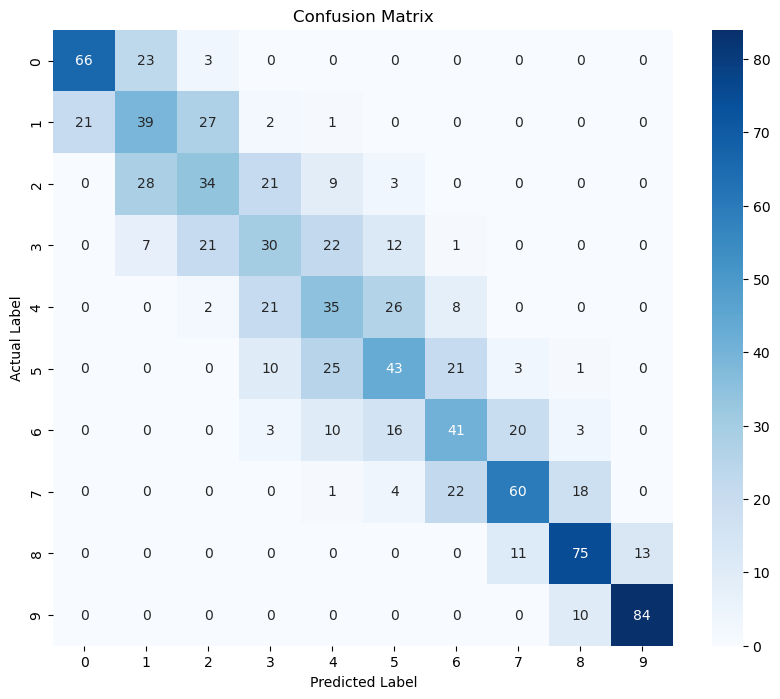
\includegraphics[scale=0.5]{ConfusionMatrix10classpercentile.png}
    \end{minipage}
    Confusion Matrix for Ensemble Model (10 Classes by Percentile): Representing a model with 10 class categories defined by percentiles, this confusion matrix evaluates the model's classification accuracy, detailing the counts of correctly and incorrectly classified instances for each class.

       \begin{minipage}{\textwidth}
        \centering
        \caption{ConfusionMatrix With Naive Bayes Manual Bucket}
        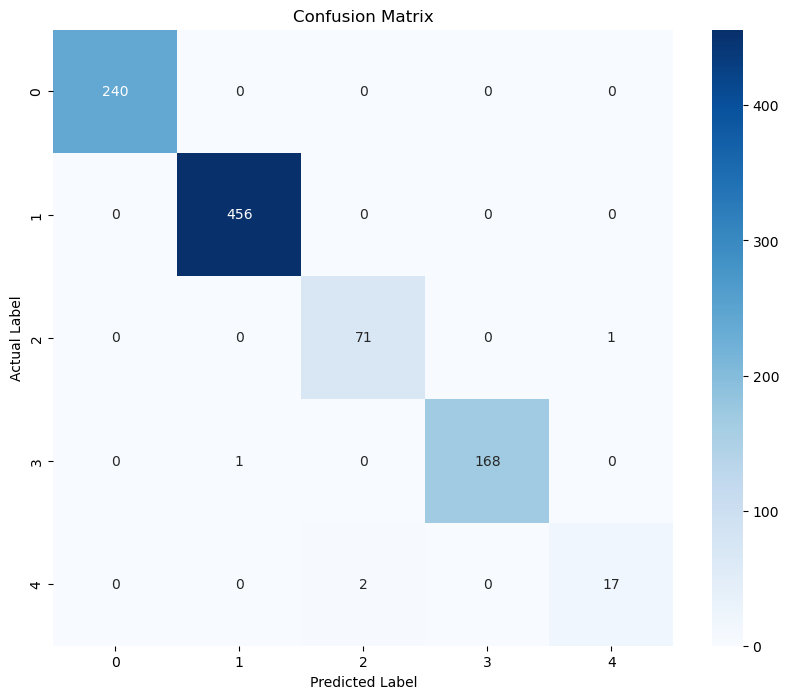
\includegraphics[scale=0.5]{Simplified Matrix by string class.png}
    \end{minipage}
    Confusion Matrix for Ensemble Model: Representing a model with 5 class categories manually defined, this confusion matrix evaluates the model's classification accuracy, detailing the counts of correctly and incorrectly classified instances for each class.
    \caption{Multiple Figures}
\end{figure}


\begin{figure}[htbp]
    \centering
    
    \begin{minipage}{\textwidth}
        \centering
        \caption{ROC Multi}
        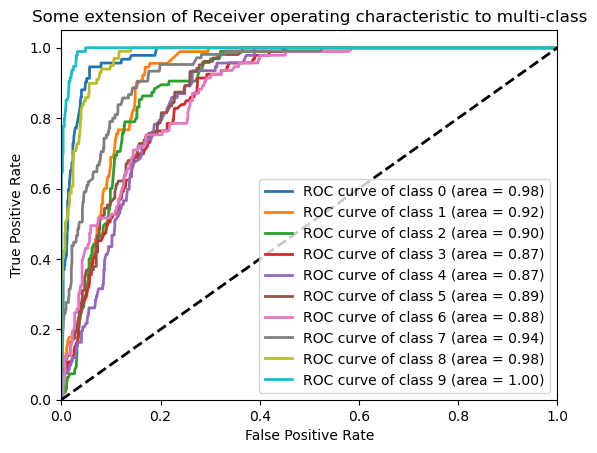
\includegraphics[scale=0.5]{ROCMulti.png}
    \end{minipage}
    
    \begin{minipage}{\textwidth}
        \centering
        \caption{ROC of cars in strings}
        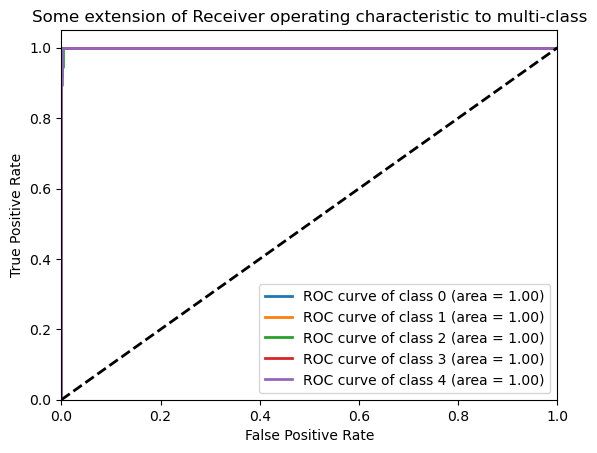
\includegraphics[scale=0.5]{ROC cars in strings.png}
    \end{minipage}
    
    
    \caption{Multiple Figures}
\end{figure}







\section{Discussion}


\subsection{Loss Metrics}

The training loss metrics for the "Wide" and "Deep" models show significant variations in performance.

- The "Wide Standard" model has the lowest training loss among the "Wide" models, indicating a strong convergence during training. It is evident that this model performed consistently well, with a decreasing loss over epochs.

- In contrast, the "Wide Regularized" model experienced a relatively high training loss in both "Deep" and "Wide" architectures compared to the other models. This suggests that the regularization techniques employed in this model might have hindered the training process.

- The "Wide Sigmoid" model performed reasonably well, with a steady decrease in training loss over epochs, indicating convergence. It falls just below the "Standard" and "Regularized" models in terms of performance for both wide and deep architectures. 

- The "Wide Tanh" models training lossremained constant over epochs in the wide and deep model with it being high in the "Wide" model and lower in the "Deep" model. This indicates that the model had difficulty learning the task and remained in a poor state. 

- The "Deep" models exhibited more variation in their validation accuracy than their "Wide" counterparts

\subsection{Accuracy Metrics}

- The " Standard" model consistently showed the highest validation accuracy among the activation functions over the training epochs. This suggests that the model not only converges well but also generalizes effectively to validation data.

- The " Regularized" model showed competitive performance, but its validation accuracy was slightly lower than the "Standard" model. The regularization might have helped prevent overfitting but at the cost of slightly lower accuracy.

- The " Sigmoid" model had a lower initial validation accuracy but managed to improve over time. It performed better than the "Tanh" model, which exhibited consistently low validation accuracy with a very low accuracy in the "Wide" architecture, indicating poor generalization.


% Summary of Results
\section{Conclusion}
\subsection{Summary of Results}

In this study, we conducted an experiment comparing two different architectures trained using the Fashion-MINST dataset. We explored "Wide" and "Deep" architectures with various activation functions, including standard, regularized, sigmoid, and tanh. 

The results indicated that the "Standard" models consistently outperformed other models, exhibiting lower training loss and higher validation accuracy. The "Regularized" models showed potential in preventing overfitting but came at a slight cost of accuracy. The "Sigmoid" models exhibited improvement over time but fall short of the "Standard" and "Regularized", while the "Tanh" model performed poorly in both architectures. The choice of activation function and architecture significantly influenced model performance.

The "Deep" and "Wide" architectures exhibited very similar results except for the "Tanh" activation. It was significantly worse in the "Wide" architecture although it underperformed the other activations in the "Deep" architecture as well. Further investigation as to why this activation underperformed so significantly may provide valuable insights. 

% Future Work
\subsection{Future Work}
If we were to continue work on this project, several avenues for further investigation and improvement could be considered:



% Table 2: Team Member Contributions
\subsection{Table 2: Team Member Contributions}
\begin{table}[h]
\centering
\begin{tabular}{|c|p{10cm}|}
\hline
\textbf{Team Member} & \textbf{Contribution} \\
\hline
Karlo Papa & Preprocessing and refinement of ML models, also drafted the report and proposal. \\
\hline
Josh Wong & Designed the ML models, developed presentation, and uploaded tables and figures into the report. \\
\hline
\end{tabular}
\end{table}



\section{Appendix}
\begin{figure}[h]
\caption{Correlation Matrix}
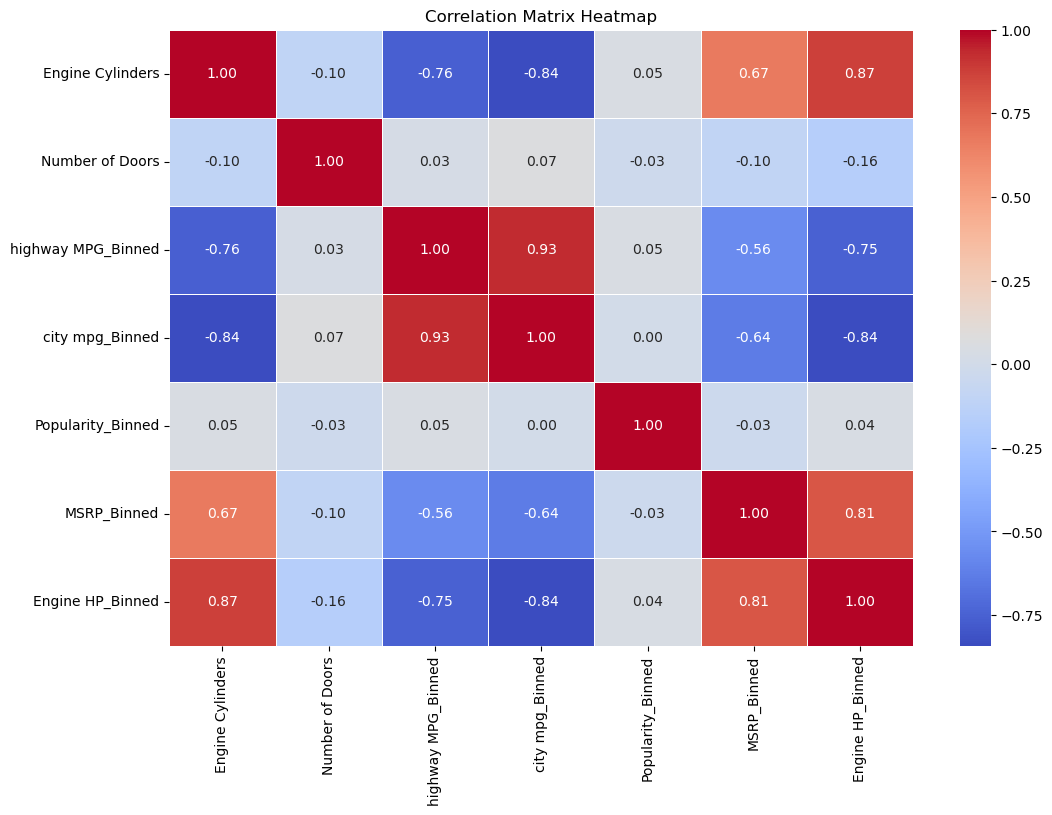
\includegraphics[scale=0.5]{CorrelationMatrix.png}\newline
\end{figure}

Correlation Matrix Heatmap: The heatmap displays the correlation coefficients between variables such as 'Engine Cylinders', 'Number of Doors', 'Highway MPG', 'City MPG', 'Popularity', 'MSRP', and 'Engine HP'. The color gradient, ranging from red for positive correlations to blue for negative correlations, visually quantifies the strength of each relationship.

\begin{figure}[h]
\caption{Decision Tree with depth of 4}
\rotatebox{90}{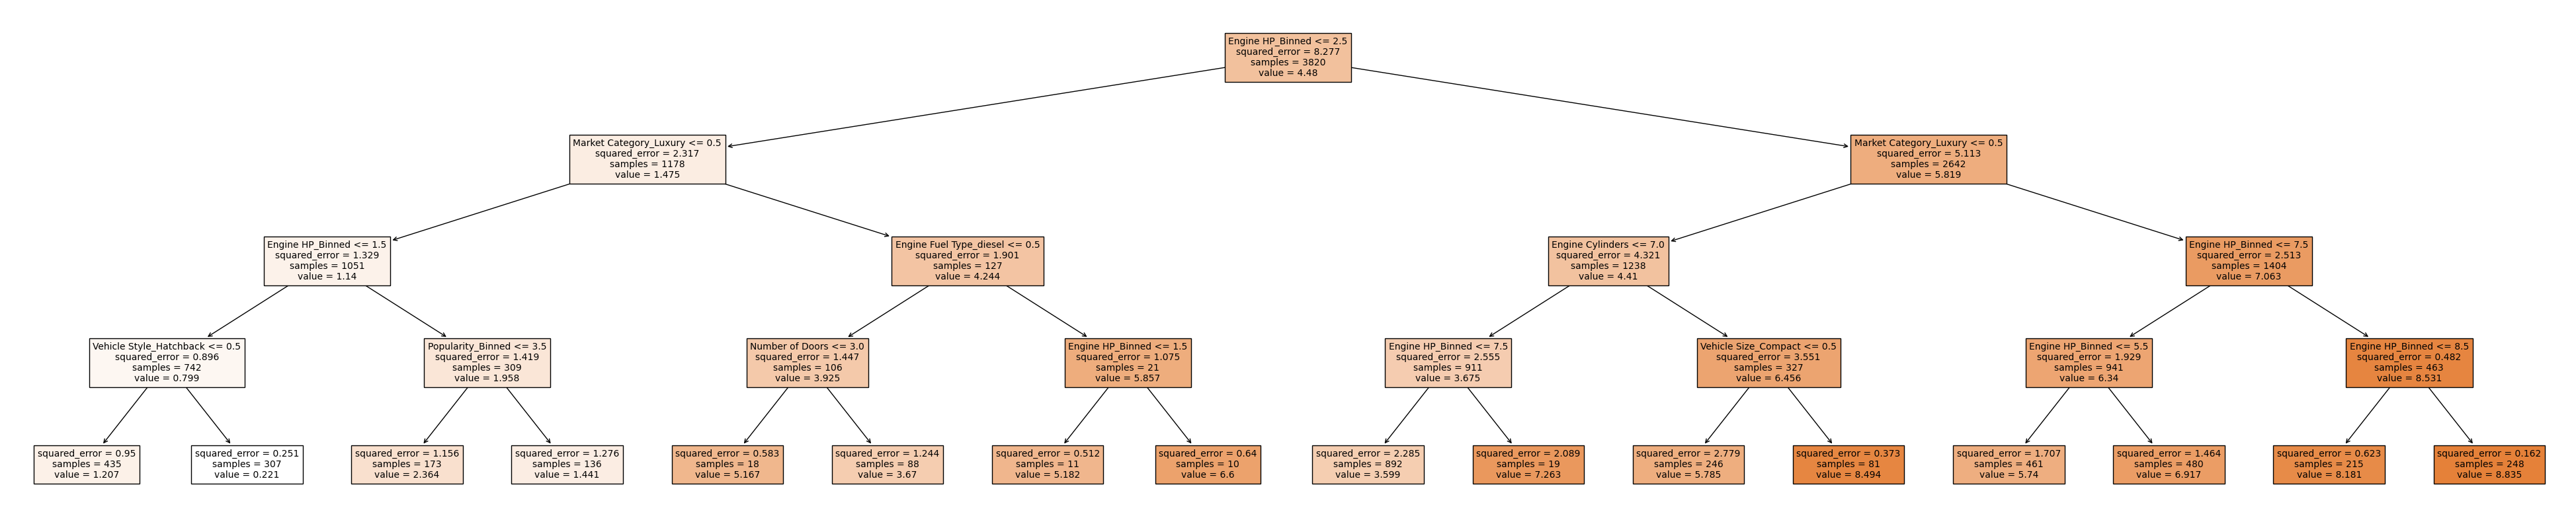
\includegraphics[scale=0.2]{4 depth.png}}
\end{figure}
Decision Tree Visualization (4 Depth): This decision tree visualization details a separate model or subset of data, with distinct decision branches and conditions, optimized for clarity in presentation. It contains a lower depth. 

\begin{figure}[h]
\caption{Decision tree with depth of 5}
\rotatebox{90}{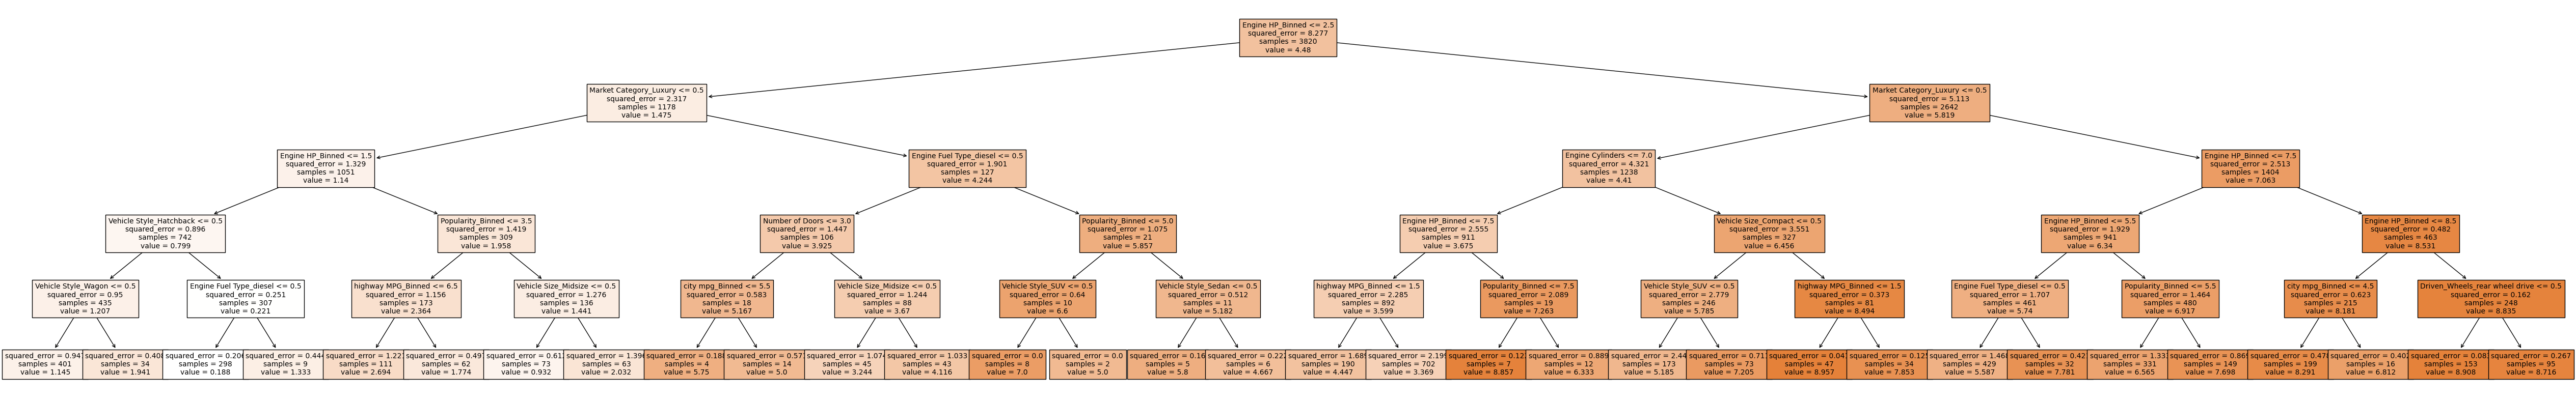
\includegraphics[scale=0.15]{5 depth.png}}
\end{figure}
Decision Tree Visualization (5 Depth): The image presents a decision tree from a machine learning model, detailing the decision-making process from the root to the leaves, based on various car feature conditions, culminating in the predicted outcomes.

\begin{figure}[h]
\caption{MSRP 2-door cars}
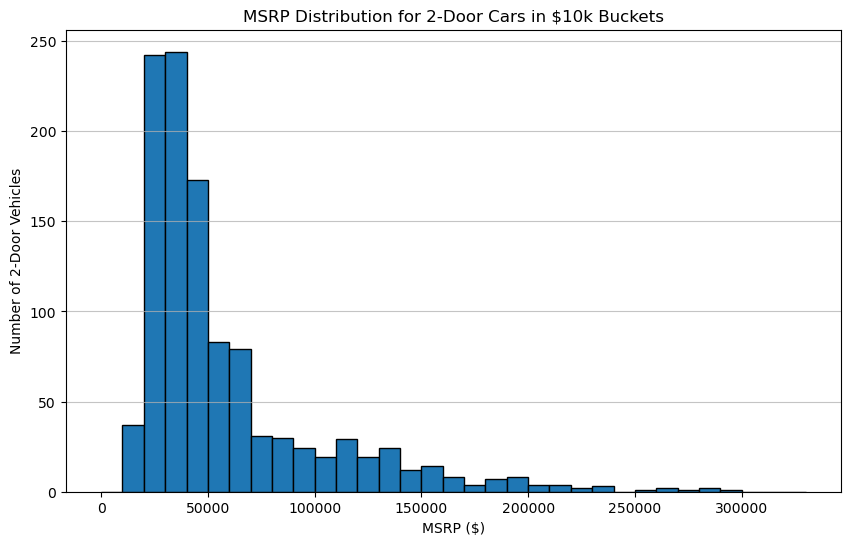
\includegraphics[scale=0.5]{MSRP 2-door 10k less.png}\newline
\end{figure}
MSRP Distribution for 2-Door Cars: This histogram narrows the focus to 2-door cars, showing their MSRP distribution and providing a price range frequency specific to this car type.
\begin{figure}[h]
\caption{MSRP 4-door cars}
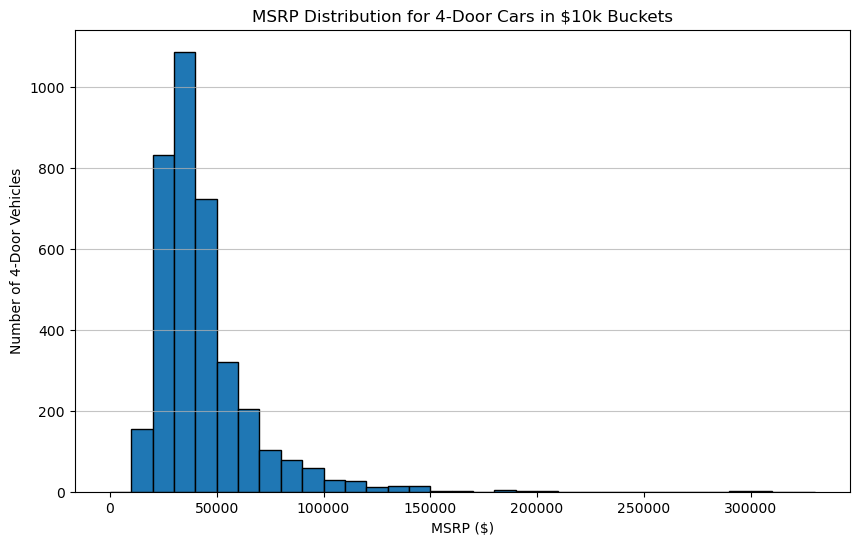
\includegraphics[scale=0.5]{MSRP 4-door 10k less.png}\newline
\end{figure}
MSRP Distribution for 4-Door Cars: The histogram presents the MSRP distribution for 4-door cars to reveal the price range frequencies for this category of vehicles.

\begin{figure}[h]
\caption{MSRP of total dataset}
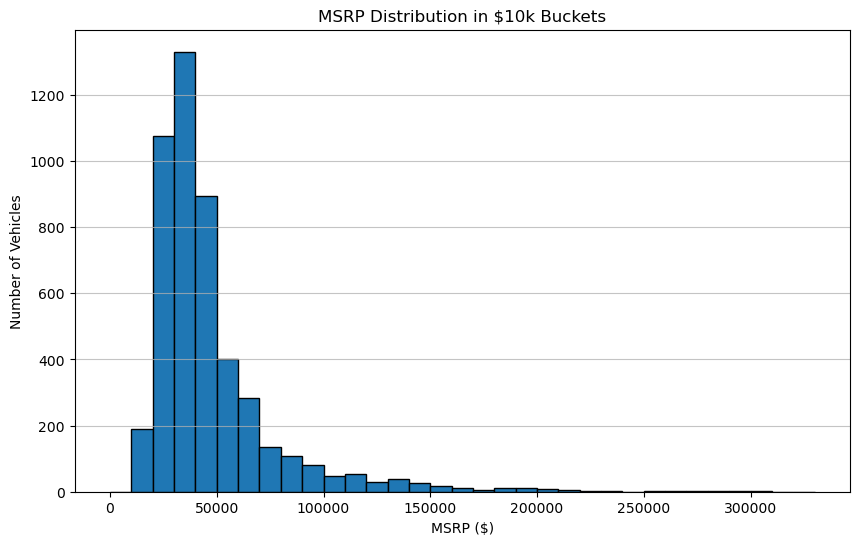
\includegraphics[scale=0.5]{MSRP 10k less.png}\newline
\end{figure}
MSRP Distribution for the whole Car dataset: The histogram illustrates the distribution of vehicle MSRPs, grouping the counts of vehicles in price intervals. It provides a clear visualization of how many vehicles fall within each price range.

\begin{figure}[h]
\caption{MSRP of dataset dropping 100k+}
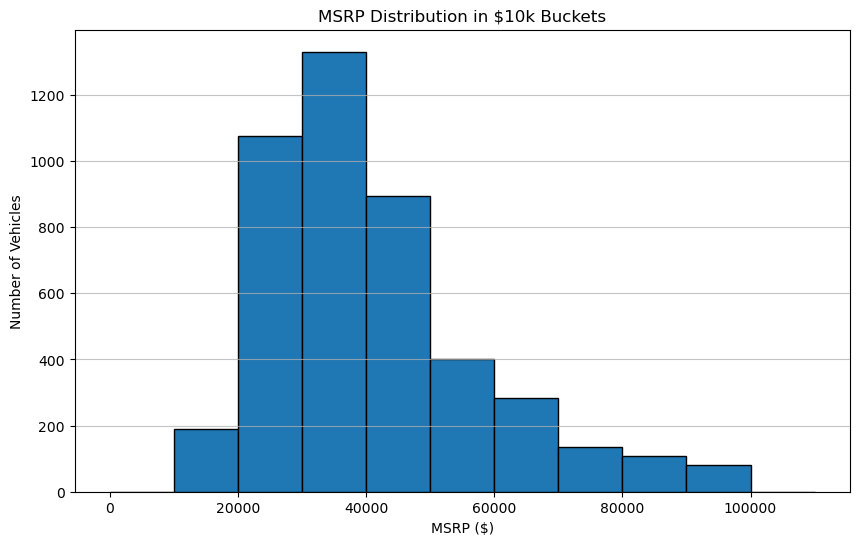
\includegraphics[scale=0.5]{MSRP in 10k.png}\newline
\end{figure}
MSRP Distribution in \$10k Buckets: The histogram illustrates the distribution of vehicle MSRPs, grouping the counts of vehicles into \$10,000 price intervals. It provides a clear visualization of how many vehicles fall within each price range. However, it doesn't contain cars over \$100k.


\section{References}
[1] Car Price PredicBon Using Machine Learning - Researchgate, www.researchgate.net/profile/A-Chandak/publicaBon/335799148\_Car\_Price\_PredicBon\_Using\_Machine\newline
\_Learning/links/61c46128c48a3d26b74b3c6e/
Car-Price-PredicBon-Using-Machine-Learning.pdf. Accessed 9 Dec. 2023.
\newline
\newline
[2] Carlier, Mathilde. “U.S.: Vehicles in OperaBon
2023.” StaBsta, 8 June 2023, www.staBsta.com/staBsBcs/859950/vehicles-in-operaBon-by-quarter-united-states/.
\newline
\newline
[3] Find a Car Brandby Country \&amp;
RegionEuropeUSAJPNGERITAUKFRAKORCHNAUSR
USESPSWEINDOtherby TagPopularLuxurySports
CarsSupercarsElectricTrucks. “Car Brands A-Z.”
CarLogos, www.carlogos.org/car-brands-a-z/.
Accessed 20 Oct. 2023.




\end{document}
